% fig_seasonal_performance.tex
% TR-24: Grouped bar chart — detection rate per scenario, fixed vs adaptive
% Y-axis: correct detections out of 3 (per scenario)
% X-axis: 4 seasonal scenarios
% Shows: fixed fails S4 (2/3), adaptive = 3/3 all
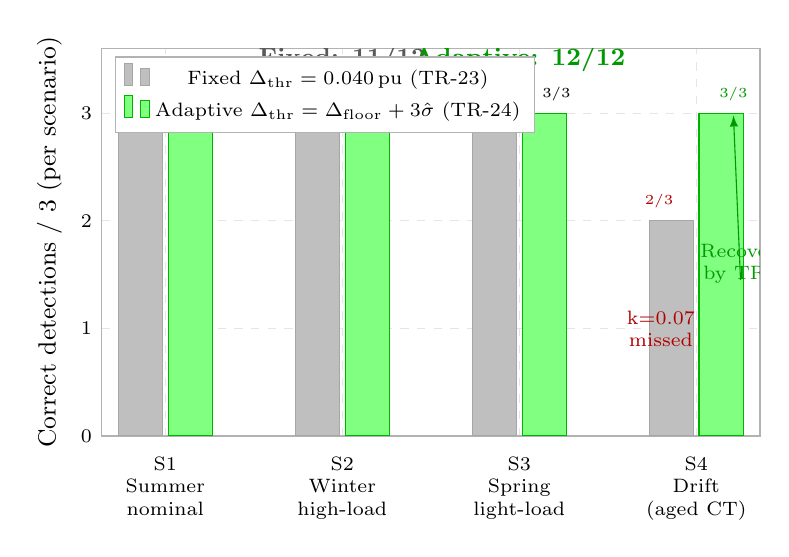
\begin{tikzpicture}
\begin{axis}[
  name         = perfax,
  ybar,
  bar width    = 16pt,
  width        = 0.82\textwidth,
  height       = 6.5cm,
  ylabel       = {Correct detections / 3 (per scenario)},
  ylabel style = {font=\small},
  ymin=0, ymax=3.6,
  ytick        = {0, 1, 2, 3},
  yticklabel style={font=\scriptsize},
  xtick        = {1, 2, 3, 4},
  xticklabels  = {S1\\Summer\\nominal,
                  S2\\Winter\\high-load,
                  S3\\Spring\\light-load,
                  S4\\Drift\\(aged CT)},
  xticklabel style={font=\scriptsize, align=center},
  enlarge x limits=0.12,
  legend style={at={(0.02,0.98)}, anchor=north west,
                font=\scriptsize, draw=gray!60},
  grid         = major,
  grid style   = {gray!20, dashed},
  tick style   = {draw=none},
  axis line style={gray!60},
]

% Fixed threshold: 3,3,3,2 (S4 misses k=0.07)
\addplot[fill=gray!50, draw=gray!70]
  coordinates { (1,3) (2,3) (3,3) (4,2) };
\addlegendentry{Fixed $\Delta_{\rm thr}=0.040$\,pu (TR-23)}

% Adaptive threshold: 3,3,3,3
\addplot[fill=green!50, draw=green!70!black]
  coordinates { (1,3) (2,3) (3,3) (4,3) };
\addlegendentry{Adaptive $\Delta_{\rm thr}=\Delta_{\rm floor}+3\hat{\sigma}$ (TR-24)}

% Value labels — fixed
\node[font=\tiny] at (axis cs:0.79, 3.18) {3/3};
\node[font=\tiny] at (axis cs:1.79, 3.18) {3/3};
\node[font=\tiny] at (axis cs:2.79, 3.18) {3/3};
\node[font=\tiny, red!70!black] at (axis cs:3.79, 2.18) {2/3};

% Value labels — adaptive
\node[font=\tiny] at (axis cs:1.21, 3.18) {3/3};
\node[font=\tiny] at (axis cs:2.21, 3.18) {3/3};
\node[font=\tiny] at (axis cs:3.21, 3.18) {3/3};
\node[font=\tiny, green!60!black] at (axis cs:4.21, 3.18) {3/3};

% Recovery annotation for S4
\node[font=\scriptsize, red!70!black, align=center]
  at (axis cs:3.80, 1.0)
  {k=0.07\\missed};

\node[font=\scriptsize, green!60!black, align=center]
  at (axis cs:4.30, 1.6)
  {Recovered\\by TR-24};
\draw[-latex, green!60!black, thin]
  (axis cs:4.25, 1.45) -- (axis cs:4.21, 2.98);

% Total summary
\node[font=\small\bfseries, gray!70!black]
  at (axis cs:2.0, 3.50)
  {Fixed: 11/12};
\node[font=\small\bfseries, green!60!black]
  at (axis cs:3.0, 3.50)
  {Adaptive: 12/12};

\end{axis}
\end{tikzpicture}
